% !TeX root = Category Theory for Algebra II.tex

\title{\textbf{Category Theory for Algebra II}}

\date{\today}
\maketitle

\begingroup
\let\clearpage\relax
\tableofcontents
\endgroup

\clearpage

\renewcommand{\nomname}{List of Symbols}
\nomenclature{$\cat{Set}$}{Category of sets and functions}
\nomenclature{$\cat{Rel}$}{Category of sets and reltaions}
\nomenclature{$\cat{Grp}$}{Category of groups and group homomorphisms}
\nomenclature{$\cat{AbGrp}$}{Category of Abelian groups and group homomorphisms}
\nomenclature{$\cat{Mon}$}{Category of monoids and monoid homomorphisms}
\nomenclature{$\cat{SemiGrp}$}{Category of semigroups and semigroup homomorphisms}
\nomenclature{$\cat{Ring}$}{Category of unital rings and unital ring homomorphisms}
\nomenclature{$\cat{Rng}$}{Category of rngs and rng homomorphisms}
\nomenclature{$\cat{Vect}_F$}{Category of vector spaces over field $F$ and linear transformations}
\nomenclature{$\cat{FinVect}_F$}{Category of finite dimensional vector spaces over field $F$ and linear transformations}
\nomenclature{$R-\cat{Mod}$}{Category of left $R$-modules}
\nomenclature{$\cat{Mod}-R$}{Category of right $R$-modules}
\nomenclature{$\Ob(\cat C)$}{Collection of objects of category $\cat C$}
\nomenclature{$\Mor(\cat C)$}{Collection of morphisms of category $\cat C$}
\nomenclature{$\Hom_{\cat C}(X, Y)$}{Collection of morphisms from $X$ to $Y$ in category $\cat C$}
\nomenclature{$\cat C\opp$}{Opposite category of category $\cat C$}
\printnomenclature[10em]

\clearpage

%\section{Introduction}\label{sec:Intro}

\section{Examples of Categories}\label{sec:CatExamples}

Before formally defining a category, we shall look at some examples of familiar categories. A category consists of a collection of \newterm{obects} and a collection of \newterm{morphisms} satisfying certain conditions that will be discussed later.
\begin{enumerate}
\item The category $\cat{Set}$ has sets as objects and functions as morphisms.
\item The collection of groups and group homomorphisms forms a category denoted by $\cat{Grp}$.
\item The collection of vector spaces over a fixed field $F$, together with $F$-linear transformations forms the category $\cat{Vect}_F$.
\item The collection of sets and relations forms the category $\cat{Rel}$.
\end{enumerate}


\section{Initial and Final Objects}\label{sec:Terminals}

An \newterm{initial object} in a category $\cat C$ is an object $A$ such that for all objects $X$ of $\cat C$, there exists a unique morphism from $A$ to $X$. A \newterm{final object} in $\cat C$ is an object $A$ such that for all objects $X$ of $\cat C$, there exists a unique morphism from $X$ to $A$. A \newterm{zero object} is an object that is both initial and final.

\begin{Example}
\begin{enumerate}
\item The empty set $\varnothing$ is the initial object and any singleton set is a final object in $\cat{Set}$.
\item The trivial group is both the initial and final object in $\cat{Grp}$.
\item The zero-dimensional vector space is the zero object in $\cat{Vect}_F$.
\item The empty set is the zero object in $\cat{Rel}$.
\end{enumerate}
\end{Example}


\section{Categories}\label{sec:Categories}

A \newterm{category} $\cat C$ is a collection $\Ob(\cat C)$ of objects and, for every two objects $X$ and $Y$ a collection $\Hom(X, Y)$ of \newterm{morphisms} or \newterm{arrows}, together with operations
\begin{equation*}
    \circ \colon \Hom(Y, Z) \times \Hom(X, Y) \to \Hom(X, Z)
\end{equation*}
for all $X, Y, Z \in \Ob(\cat C)$, satisfying the following:
\begin{enumerate}[label=(C\arabic*)]
\item $\Hom(X_1, Y_1)$ and $\Hom(X_2, Y_2)$ are disjoint unless $X_1 = X_2$ and $Y_1 = Y_2$.
\item For each $X \in \Ob(\cat C)$, there exists an \newterm{identity morphism} $\id_X$ or $1_X$ such that if $f \in \Hom(X, Y)$, there $f \circ \id_X = f$ and if $g \in \Hom(Z, X)$, then $\id_X \circ g = g$.
\item If $F \in \Hom(X, Y)$, $g \in \Hom(Y, Z)$, and $h \in \Hom(Z, W)$, then
\begin{equation*}
    h \circ (g \circ f) = (h \circ g) \circ f.
\end{equation*}
This is the \newterm{law of associativity}.
\end{enumerate}

The collection of all morphisms of $\cat C$ is denoted by $\Mor(\cat C)$. If $f \in \Hom(X, Y)$, then we write $f \colon X \to Y$ or $\xymatrix{X \ar[r]^f & Y}$ and say that $f$ is a \newterm{morphism from $X$ to $Y$}, or that $X = \dom f$ is the \newterm{domain} and $Y = \cod f$ is the codomain of $f$.

\begin{Example}\label{ex:Categories}
\begin{enumerate}
\item\label{it:Categories2IsoObj} $\cat C = \{X, Y\}$, $\Mor(\cat C) = \{1_X, 1_Y, f \colon X \to Y, g \colon Y \to X \}$ with $1_X$ and $1_Y$ as identity morphisms and $f \circ g = 1_Y$, $g \circ f = 1_X$. Graphically,
\begin{equation*}
\boxed{\xymatrix{
X \ar @(ld, lu)^{1_X} \ar @/^/[r]^f & Y \ar @(ru, rd)^{1_Y} \ar @/^/[l]^g
}}
\end{equation*}

\item\label{it:Categories1ObjDisc} $\cat C = \{\bullet\}$, $\Mor(\cat C) = \{1\}$.

\item\label{it:CategoriesRing} $\cat{Ring}$ is the category of unital rings and unital ring homomorphisms.

\item\label{it:CategoriesMon} $\cat{Mon}$ is the category of monoids and monoid homomorphisms.

\item\label{it:CategoriesTop} $\cat{Top}$ is the category of topological spaces and continuous maps.

\item\label{it:CategoriesAbGrp} $\cat{AbGrp}$ is the category of Abelian groups and group homomorphisms.
\end{enumerate}
\end{Example}

\begin{Exercise}
\begin{enumerate}
\item In the category $\cat C$ given below, determine the compositions of all the non-identity morphisms.
\begin{equation*}
\boxed{\xymatrix{
	X \ar @(l, u)^{1_X} \ar @<+0.5ex>[rr]^f \ar @<-0.5ex>[rr]_g  \ar [dr]_k && Y \ar @(u, r)^{1_Y}  \ar[ld]^h \\
	& Z \ar @(dr, dl)^{1_Z} 
}}
\end{equation*}

\item In the category $\cat C$ given below, determine the compositions of all the non-identity morphisms.
\begin{equation*}
\boxed{\xymatrix{
	X \ar @(l, u)^{1_X} \ar @/^/[dr]^h && Y \ar @(u, r)^{1_Y} \ar[ll]_f \ar[ld]^g \\
	& Z \ar @(dr, dl)^{1_Z} \ar @/^/[ul]^k
}}
\end{equation*}

\item If $\cat C$ is a category with $\Ob(\cat C) = \{ \bullet \}$ and $\Mor(\cat C) = \{1, f, g\}$, such that $f \circ g = 1$. Then determine $f \circ f$, $g \circ g$, and $g \circ f$.

\item Show that the following is not a valid category.
\begin{equation*}
\boxed{\xymatrix{
	X \ar @(ld, lu)^{1_X} \ar  @/^1pc/[rr]^f  \ar  @/_1pc/[rr]_h && Y \ar @(ru, rd)^{1_Y}  \ar[ll]|-g
}}
\end{equation*}

\item Let $X$ be an object of a category $\cat C$. Denote by $\cat C / X$ the category whose objects are
\begin{equation*}
\Ob(\cat C / X) = \qty{\, f \colon Y \to X \mid Y \in \Ob(\cat C) \,}
\end{equation*}
morphisms are
\begin{equation*}
\Hom(f, g) = \qty{\, h \colon Y \to Z \mid g \circ h = f \,}
\end{equation*}
for all $Y, Z \in \Ob(\cat C)$, $f \colon Y \to X$, $g \colon Z \to X$, and the composition of $m \in \Hom(f, g)$ and $n \in \Hom(g, h)$ is defined to be the morphism $n \circ m$ of $\cat C$ . Show that $\cat C / X$ is indeed a category.

\item Define a category $X / \cat C$ analogous to $\cat C / X$ and show that it is a category.

\item Let $\cat C$ be a category. Define a new category $\cat C\opp$ whose objects are the same as those of $\cat C$, with a morphism $f\opp \colon Y \to X$ corresponding to every morphism $f \colon X \to Y$ in $\cat C$, and composition defined by
\begin{equation*}
f\opp \circ g\opp = (g \circ f)\opp
\end{equation*}
for all $f\opp \colon Y \to X$, $g\opp \colon Z \to Y$. Show that $\cat C\opp$ is indeed a category (see \cref{sec:Duality}).

\item What is the category $(\cat C / X)\opp$?

\item Can the following be a category? If so, how?
\begin{equation*}
\boxed{\xymatrix{
	& \bullet \ar @(ru, lu)_f \ar @(ld, rd)_1 &
}
}
\end{equation*}

\item Can the following be a category? If so, how?
\begin{equation*}
\boxed{\xymatrix{
	X \ar @(ld, lu)^{1_X} \ar  @/^1pc/[rr]^f  \ar  @/_1pc/[rr]_h && Y \ar @(ul, ur)^k \ar @(ur, dr)^{1_Y} \ar[ll]|-g
}}
\end{equation*}

\item Can the following be a category? If so, how?
\begin{equation*}
\boxed{\xymatrix{
	X \ar @(ld, lu)^{1_X} \ar  @/^1pc/[rr]^f  \ar  @/_1pc/[rr]_h && Y \ar @(ul, ur)^k \ar @(ur, dr)^{1_Y} \ar @(dr, dl)^l \ar[ll]|-g
}}
\end{equation*}
\end{enumerate}
\end{Exercise}

A category is \newterm{small} if its collections of objects and morphisms are sets -- note that this is equivalent to simply saying that its collection of morphisms, as the objects are in one-to-one correspondence with the identity morphisms. A category that is not small is \newterm{large}. A category is \newterm{locally small} if $\Hom(X, Y)$ is a set for every two objects $X$ and $Y$ of the category. In this case, $\Hom(X, Y)$ is said to be a \newterm{hom-set}.

In \cref{ex:Categories}, the categories given in \labelcref{it:Categories2IsoObj,it:Categories1ObjDisc} are small (and hence also locally small), whereas the ones given in \labelcref{it:CategoriesRing,it:CategoriesMon,it:CategoriesAbGrp} are large but locally small.

\section{Duality}\label{sec:Duality}
The \newterm{opposite category} of a category $\cat C$ is the category $\cat C\opp$ with $\Ob(\cat C\opp) = \Ob(\cat C)$ and for each pair of objects $X$ and $Y$, $\Hom_{\cat C\opp}(X, Y) = \qty{\, f\opp \mid f \in \Hom_{\cat C}(Y, X) \,}$, in which composition is defined as
\begin{equation*}
g\opp \circ f\opp = (f \circ g)\opp
\end{equation*}
for all $f\opp \in \Hom_{\cat C\opp}(X, Y)$ and $g\opp \in \Hom_{\cat C\opp}(Y, Z)$, for all objects $X$, $Y$, and $Z$.

The fact that $\cat C\opp$ is a category gives rise to the principle of duality -- if a statement is true in all categories, then its \newterm{dual statement}, obtained by reversing the directions of all morphisms, must also be true in all categories. In fact, every concept defined in category theory has a dual concept. For instance, the concepts of initial and final objects are duals of each other. We will later prove that any two initial objects in a category must be isomorphic to each other. From this, it immediately follows, by the principle of duality, that any two final objects in a category must be isomorphic to each other.


\section{Diagram Chasing}\label{sec:DiagramChasing}

A diagram of objects and morphisms \newterm{commutes} (or is \newterm{commutative}) if, whenever there are two directed paths with the same source and same target, the composition of the morphisms along one path equals the composition of the morphisms along the other. That is, for each pair of paths
\begin{equation*}
\xymatrix{
& \bullet \ar[r]^{f_2} &  \bullet & \cdots & \bullet \ar[r]^{f_{m-1}} & \bullet \ar[rd]^{f_m} & \\
\bullet \ar[ru]^{f_1} \ar[rd]_{g_1} &&&&&& \bullet \\
& \bullet \ar[r]_{g_2} & \bullet & \cdots & \bullet \ar[r]_{g_{n-1}} & \bullet \ar[ru]_{g_n} &
}
\end{equation*}
in the diagram, $f_m \circ f_{m-1} \circ \cdots \circ f_2 \circ f_1 = g_n \circ g_{n-1} \circ \cdots \circ g_2 \circ g_1$.

\begin{Example} In the diagram below, suppose $h = g \circ f$.
\begin{equation*}
\xymatrix{
X \ar[r]^f \ar[d]_h & Y \ar[d]^{1_Y} \\
Z & Y \ar[l]^g
}
\end{equation*}
In this diagram, there are two different directed paths from $X$ to $Z$, one consisting of the morphisms $f$, $1_Y$, and $g$, and the other consisting of a single morphism $h$. The composition of the morphisms along the first path is $g \circ 1_Y \circ f = g \circ f = h$, and the composition of the morphisms along the second path is simply $h$. As both of these are equal, the diagram commutes.
\end{Example}

\begin{Example}
Consider $f \colon \mathbb C \to \mathbb C$, $f(z) = -iz$, $g \colon \mathbb C \to \mathbb R$, $g(z) = \Re(z)$, and $h \colon \mathbb C \to \mathbb R$, $h(z) = \Im(z)$, for all $z \in \mathbb C$. Then the following diagram commutes:
\begin{equation*}
\xymatrix{
\mathbb C \ar[r]^f \ar[rd]_h & \mathbb C \ar[d]^g \\
& \mathbb C
}
\end{equation*}
To verify this, we could take an arbitrary element of $\mathbb C$ and ``chase'' it across the diagram to see if it maps to the same element along all paths that lead to the same target. We may represent this visually as given below.
\begin{equation*}
\xymatrix@C=3.2em{
x + iy \ar@{|->}[r]^{(-i) \times \leftrightline} \ar@{|->}[rd]_{\Im} & y - ix \ar@{|->}[d]^{\Re} \\
& y
}
\end{equation*}
\end{Example}

\begin{Exercise}
Let $f \colon \mathbb C \to \mathbb C$, $f(z) = \overline z$, $g \colon \mathbb C \to \mathbb C$, $g(z) = z^2$, and $h \colon \mathbb C \to \mathbb C$, $h(z) = \Re(z)$. Which of the following is/are commutative?
\begin{figure}[H]
\centering
\subcaptionbox{}{
	$\xymatrix{
	 	\mathbb C \ar[r]^f \ar[d]_g & \mathbb C \ar[d]^g \\
 	 	\mathbb C \ar[r]_f & \mathbb C 
 	}$
} \qquad
\subcaptionbox{}{
	$\xymatrix{
		\mathbb C \ar[r]^f \ar[d]_h & \mathbb C \ar[d]^{h} \\
		\mathbb C \ar[r]_f & \mathbb C 
	}$
}
\end{figure}
\end{Exercise}

\begin{Example}
The law of associativity of composition can be stated in terms of a commutative diagrams as follows. For all morphisms $f$, $g$, $h$ with domains and codomains as shown in the diagram below, if each subdiagram with three vertices commutes, then the whole diagram commutes.
\begin{equation*}
\xymatrix{
\bullet \ar[r]^f \ar@/^2pc/[rr] \ar@/^3pc/[rrr]^{} \ar@/_3pc/[rrr]_{}
& \bullet \ar[r]^g \ar@/_2pc/[rr]
& \bullet \ar[r]^h & \bullet
}
\end{equation*}

The identity morphism of an object $X$ can be defined as the morphism such that all diagrams of the following form commute.
\begin{equation*}
\xymatrix@=3em{
X \ar[r]^f \ar[rd]^{1_X} \ar[d]_g & Y \ar[d]^f \\
Z \ar[r]_g & X
}
\end{equation*}
\end{Example}

Very often, the commutativity of a larger diagram can be checked by verifying the commutativity of its smaller components. Commutative diagrams of the forms given below are called \newterm{commuting triangles} and \newterm{commuting squares}, respectively.
\begin{align*}
\xymatrix{
\bullet \ar[r] \ar[rd] & \bullet \ar[d]\\
& \bullet
}
&&
\xymatrix{
\bullet \ar[r] \ar[d] & \bullet \ar[d] \\
\bullet \ar[r] & \bullet
}
\end{align*}

\begin{Exercise}[{\cite[Exercise 1.2]{SchalkSimmons2005}}]
In each of the diagrams given below, show that if the two triangles commute, then the square commutes.
\begin{figure}[H]
\centering
\subcaptionbox{\label{subfig:CommSq1}}{
$\xymatrix@=3em{
\bullet \ar[r] \ar[d] \ar[rd] & \bullet \ar[d] \\
\bullet \ar[r] & \bullet
}$
}
\hspace{0.3\textwidth}
\subcaptionbox{\label{subfig:CommSq2}}{
$\xymatrix@=3em{
\bullet \ar[r] \ar[d] & \bullet \ar[d] \ar[ld]\\
\bullet \ar[r] & \bullet
}$
}
\end{figure}
\end{Exercise}

\begin{Solution*}
In \subref{subfig:CommSq1}, from the commutativity of the upper triangle, the composition of the top and right sides of the square equals the diagonal, which, from the commutativity of the lower triangle, equals the composition of the left and bottom sides. This shows that the square commutes.

In \subref{subfig:CommSq2}, since the lower triangle commutes, the right side equals the composition of the diagonal and the bottom side. Hence, the composition of the top and right sides equals the composition of the top side, the diagonal, and the bottom side. Similarly, from the commutativity of the upper triangle, the composition of the top side, the diagonal, and the bottom side also equals the composition of the bottom and left sides. Thus, the square commutes.
\end{Solution*}

\note{Arguments such as the above one are much easier to \emph{see} than to understand by reading, but this requires some training. The writing itself could be made considerably simpler by naming the arrows (the morphisms) in the diagram and expressing the argument in the form of equations, but the aim of these exercises is to develop the skill of ``diagram chasing''. Attempt the remaining exercises in the same manner, avoiding the urge to name arrows, as much as possible.}

\begin{Exercise}[{\cite[Exercise 1.2]{SchalkSimmons2005}}]
In the diagram given below, viewed as a tetrahedron, show that if the left, right, and bottom faces commute, then the back face also commutes.
\begin{equation*}
\xymatrix@=3em{
& \bullet \ar[ld] \ar[dd] \ar[rd] & \\
\bullet \ar[rd] \ar[rr]|\hole & & \bullet \\
& \bullet \ar[ru] &
}
\end{equation*}
\end{Exercise}

\begin{Exercise}
In each of the diagrams below, show that if both the squares commute, then the outer rectangle commutes.
\begin{figure}[H]
\centering
\subcaptionbox{}{$\xymatrix@=3em{
\bullet \ar[r] \ar[d] & \bullet \ar[r] \ar[d] & \bullet \ar[d] \\
\bullet \ar[r] & \bullet \ar[r] & \bullet
}$}
\hspace{0.1\textwidth}
\subcaptionbox{}{$\xymatrix@=3em{
\bullet \ar[r] \ar[d] & \bullet \ar[r] \ar[d] & \bullet \\
\bullet \ar[r] & \bullet \ar[r] & \bullet \ar[u]
}$}
\hspace{0.1\textwidth}
\subcaptionbox{}{$\xymatrix@=3em{
\bullet \ar[r] \ar[d] & \bullet \ar[r] & \bullet \ar[d] \\
\bullet \ar[r] & \bullet \ar[r] \ar[u] & \bullet
}$}
\end{figure}
\end{Exercise}

\begin{Exercise}
Show that if the inner triangle and the three trapeziums in the diagram below commute, then the outer triangle commutes.
\begin{equation*}
\xymatrix{
&&& \bullet \ar[d] \ar[rrrddd] &&& \\
&&& \bullet \ar[rd] &&& \\
&& \bullet \ar[ur] \ar[rr] && \bullet \ar[rrd] && \\
\bullet \ar[rrruuu] \ar[rru] \ar[rrrrrr] &&&&&& \bullet
}
\end{equation*}
\end{Exercise}

\begin{Exercise}[{\cite[Exercise 1.4]{SchalkSimmons2005}}]
Show that if the inner square and the four trapeziums in the diagram below commute, then the outer square commutes.
\begin{equation*}
\xymatrix@=2.5em{
\bullet \ar[ddd] \ar[rd] \ar[rrr] &&& \bullet \ar[ld] \ar[ddd] \\
& \bullet \ar[d] \ar[r] & \bullet \ar[d] & \\
& \bullet \ar[r] & \bullet \ar[rd] & \\
\bullet \ar[ru] \ar[rrr] &&& \bullet
}
\end{equation*}
\end{Exercise}

\begin{Exercise}
Let $G$ and $H$ be groups. If $f \colon G \to H$ is any function, defined $f \times f \colon G \times G \to H \times H$ by $f(x, y) = (f(x), f(y))$, for all $x, y \in G$. Let $\cdot$ and $*$ denote the group operations in $G$ and $H$, respectively. Then show that $f$ is a homomorphism if and only if the following diagram commutes.
\begin{equation*}
\xymatrix@C=5em@R=4em{
G \times G \ar[r]^{f \times f} \ar[d]_\cdot & H \times H \ar[d]^{*} \\
G \ar[r]_f & H
}
\end{equation*}
\end{Exercise}

\begin{Exercise}
Show that in the diagram below, if all the parallelograms commute, and any one of the two squares commutes, then all directed paths with three arrows are equal under composition.
\begin{equation*}
\xymatrix@=3em{
& \bullet \ar[r] \ar[rd] & \bullet \ar[rd] & \\
\bullet \ar[r] \ar[rd] \ar[ru] & \bullet \ar[rd] \ar[ru] & \bullet \ar[r] & \bullet \\
& \bullet \ar[r] \ar[ru] & \bullet \ar[ru] &
}
\end{equation*}
\end{Exercise}

\section{Some Classes of Morphisms}\label{sec:MorphismClasses}

A morphism $f \colon X \to Y$ in a category $\cat C$ is an \newterm{isomorphism} if there exists a morphism $g \colon Y \to X$ in $\cat C$ such that $g \circ f = 1_X$ and $f \circ g = 1_Y$. Such a morphism $g$ is an \newterm{inverse} of $f$. If there exists an isomorphism $f \colon X \to Y$, then $X$ is \newterm{isomorphic} to $Y$, written $X \cong Y$.

Equivalently, we can define an isomorphism as a morphism $f$ such that there exists a morphism $g$ making the following diagram commute.
\begin{equation*}
\xymatrix@C=2.5em{
Y \ar[r]^g \ar@/^2.2pc/[rr]^{1_Y} & X \ar[r]^f \ar@/_2.2pc/[rr]_{1_X} & Y \ar[r]^g & X
}
\end{equation*}

\begin{Exercise}
\begin{enumerate}
\item Show that each identity morphism is an isomorphism.
\item Show that if $f$ is an isomorphism, then it has a unique inverse, and the inverse is also an isomorphism.
\item Show that the composition of two compatible isomorphisms is also an isomorphism.
\item Show that the isomorphism relation $\cong$ is an equivalence relation on the collection of objects of a category.
\end{enumerate}
\end{Exercise}

\begin{Example}
\begin{enumerate}
\item In $\cat{Set}$, the isomorphisms are exactly the bijective functions.
\item In $\cat{Grp}$, $\cat{Mon}$, $\cat{Ring}$, and $\cat{AbGrp}$, the isomorphisms are the bijective homomorphisms of the respective algebraic structures.
\item In $\cat{Vect}_F$, the isomorphisms are the bijective linear transformations.
\item In $\cat{Top}$, the isomorphisms are the homeomorphisms. Note that a homeomorphism is not simply a bijective continuous map (i.e.\ a morphism of $\cat{Top}$ that is bijective as a function). Why?
\item In the category given in \cref{ex:Categories}, \labelcref{it:Categories2IsoObj}, all the morphisms are isomorphisms.
\end{enumerate}
\end{Example}

We may weaken the definition of isomorphism in two ways as follows. If $r \colon X \to Y$ and $s \colon Y \to X$ are morphisms such that $r \circ s = 1_Y$, then $r$ is a \newterm{retraction} and $s$ is a \newterm{section}.
\begin{equation*}
\xymatrix{
Y \ar[r]^s \ar[rd]_{1_Y} & X \ar[d]^r \\
& Y
}
\end{equation*}
We also say that $r$ is a \newterm{left inverse} of $s$ and that $s$ is a \newterm{right inverse} of $r$. Thus, a retraction is a right-invertible morphism and a section is a left-invertible morphism.

\begin{Exercise}
Prove that a morphism is an isomorphism if and only if it is both a retraction and a section.

\note{The statement that a morphism is both a retraction and a section only tells you that it has some right inverse and some left inverse -- not that the right and left inverses are the same. That is, if $f \colon X \to Y$ is both a retraction and a section, you may only assume that there exist morphisms $s \colon Y \to X$ and $r \colon Y \to X$ such that $f \circ s = 1_Y$ and $r \circ f = 1_X$.}

\hint{Show that $r = s$.}
\end{Exercise}

\begin{Example}\label{ex:SetRetSec}
In the category $\cat{Set}$, consider the sets $X = \mathbb R$ and $Y = \mathbb Z$. Define $r \colon X \to Y$ by $r(x) = \floor x$ (the greatest integer not exceeding $x$) for all $x \in X$, and $s \colon Y \to X$ by $s(y) = y$ for all $y \in Y$. Then $r \circ s = \id_Y$. Note that neither $r$, nor $s$ is an isomorphism.
\end{Example}

\begin{Exercise}
\begin{enumerate}
\item Show that $f$ is a retraction in a category $\cat C$ if and only if $f\opp$ is a section in $\cat C\opp$.
\item Show that in $\cat{Set}$, every section is an injective function and every retraction is a surjective function.
\item Show that in $\cat{Set}$, every injective function is a section.
\item Read about the Axiom of Choice and try to understand its equivalence to the following statement: In $\cat{Set}$, every surjective function is a retraction.
\item Show that in $\cat{Grp}$, every section is an injective group homomorphism.
\item In $\cat{Grp}$, consider the inclusion map $\iota \colon \mathbb Z \to \mathbb R$ defined by $\iota(n) = n$ for all $n \in \mathbb Z$ (where $\mathbb Z$ and $\mathbb R$ are the additive groups defined as usual). Show that $\iota$ is an injective homomorphism, but is not a section.
\end{enumerate}
\end{Exercise}

The definitions of sections and retractions can be further weakened in the following manner. A \newterm{monomorphism} is a morphism $m \colon X \to Y$ such that for all $Z$ and $f, g \colon Z \to X$, if $m \circ f = m \circ g$, then $f = g$. In other words, $m$ is \newterm{left-cancellable}. We also say that $m$ is \newterm{monic}. Dually, an \newterm{epimorphism} is a morphism $e \colon X \to Y$ such that for all $Z$ and $f, g \colon Y \to Z$, if $f \circ e = g \circ e$, then $f = g$. That is, $e$ is \newterm{right-cancellable}. We also say that $e$ is \newterm{epic}.

\begin{Exercise}
Show that monomorphisms and epimorphisms are indeed dual concepts.
\end{Exercise}

Observe that the defining property of a monomorphism, namely $m \circ f = m \circ g \implies f = g$, appears similar to that of an injective functions between sets, namely $m(x) = m(y) \implies x = y$ (for elements $x$ and $y$ of the domain). Indeed, monomorphisms are the categorical generalisations of injective functions. This idea is formalised in the statement of the next exercise.

\begin{Exercise}
Show that monomorphisms in the category $\cat{Set}$ are exactly injective functions.
\end{Exercise}

\begin{Solution*}
Consider a function $m \colon X \to Y$ in $\cat{Set}$. First, suppose that $m$ is a monomorphism. That is, if $f$ and $g$ are functions from some set $Z$ to $X$ such that $m \circ f = m \circ g$, then $f = g$. We need to show that $m$ is an injection. That is, if $x$ and $y$ are two elements of $X$ such that $m(x) = m(y)$, then $x = y$. Let $Z$ be a singleton set, say $Z = \{\bullet\}$. Define functions $f, g \colon Z \to X$ by $f(\bullet) = x$ and $g(\bullet) = y$.
\begin{center}
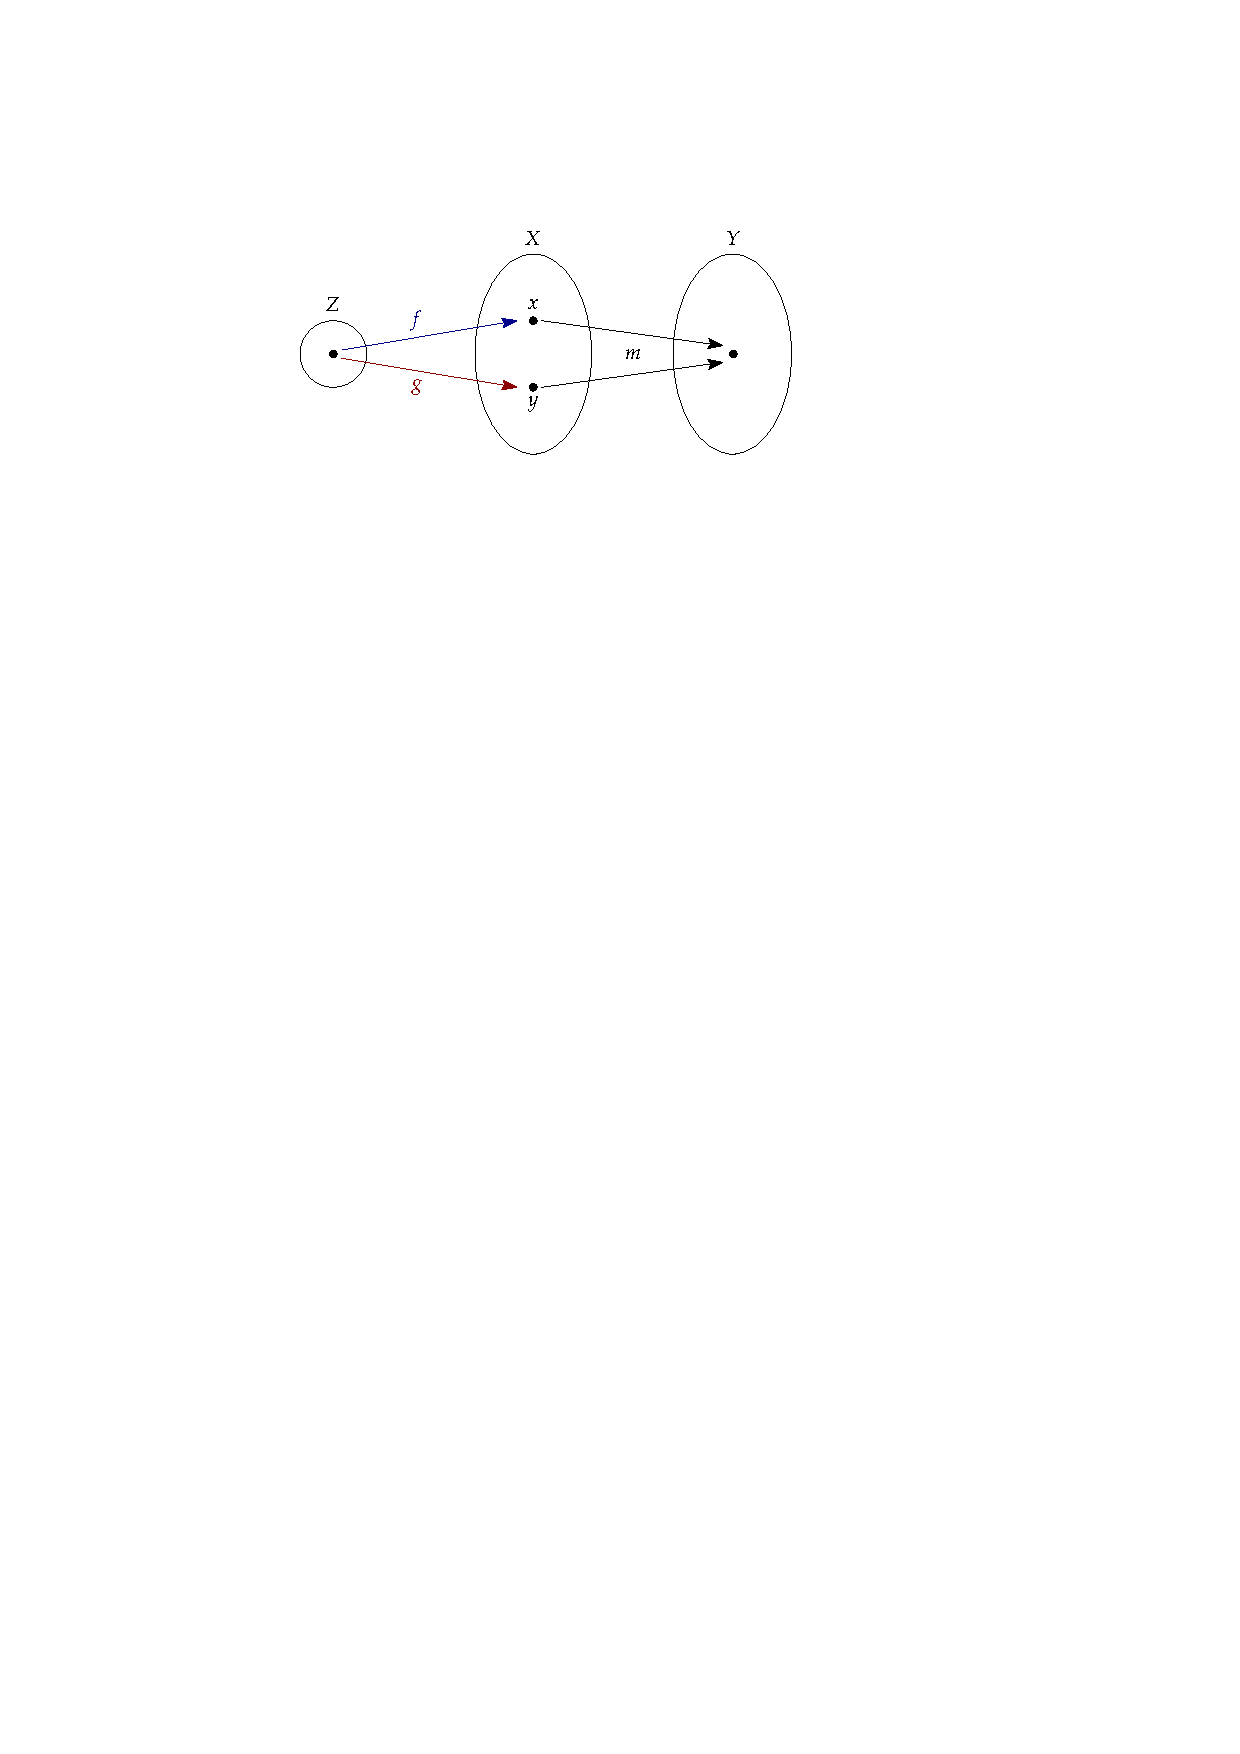
\includegraphics[scale=1.2]{Mono=Injection.pdf}
\end{center}
Then, $m(f(\bullet)) = m(x)$, and $m(g(\bullet)) = m(y)$. Now, suppose that $m(x) = m(y)$. Then we have $m(f(\bullet)) = m(g(\bullet))$, which implies that $m \circ f = m \circ g$ (since $\bullet$ is the only element of the domain $Z$ of these two functions). But $m$ is a monomorphism, and therefore we have $f = g$, which implies $f(\bullet) = g(\bullet)$, i.e. $x = y$, as required.

Next, suppose that $m$ is an injection. If $f, g \colon Z \to X$ are such that $m \circ f = m \circ g$, then for all $z \in Z$, $m(f(z)) = m(g(z))$. As $m$ is injective, this implies that $f(z) = g(z)$, for all $z \in Z$, i.e. $f = g$, showing that $m$ is a monomorphism.
\end{Solution*}

Similarly, epimorphisms are the categorical generalisations of surjective functions, as you are asked to show in the next exercise.

\begin{Exercise}
Show that epimorphisms in the category $\cat{Set}$ are exactly surjective functions.
\end{Exercise}



\bibliographystyle{plain}
\bibliography{References.bib}